\documentclass{amsart}

\usepackage{tikz}

\tikzstyle{node}=[circle, draw]

\tikzstyle{up}=[node, fill = red]
\tikzstyle{c1}=[node, fill = black]
\tikzstyle{md}=[node, fill = orange]
\tikzstyle{c2}=[node, fill = black]
\tikzstyle{dn}=[node, fill = yellow]
\tikzstyle{ds}=[node, fill = blue]
\tikzstyle{ex}=[node, fill = green]
\tikzstyle{nd}=[rectangle, draw]

\begin{document}
	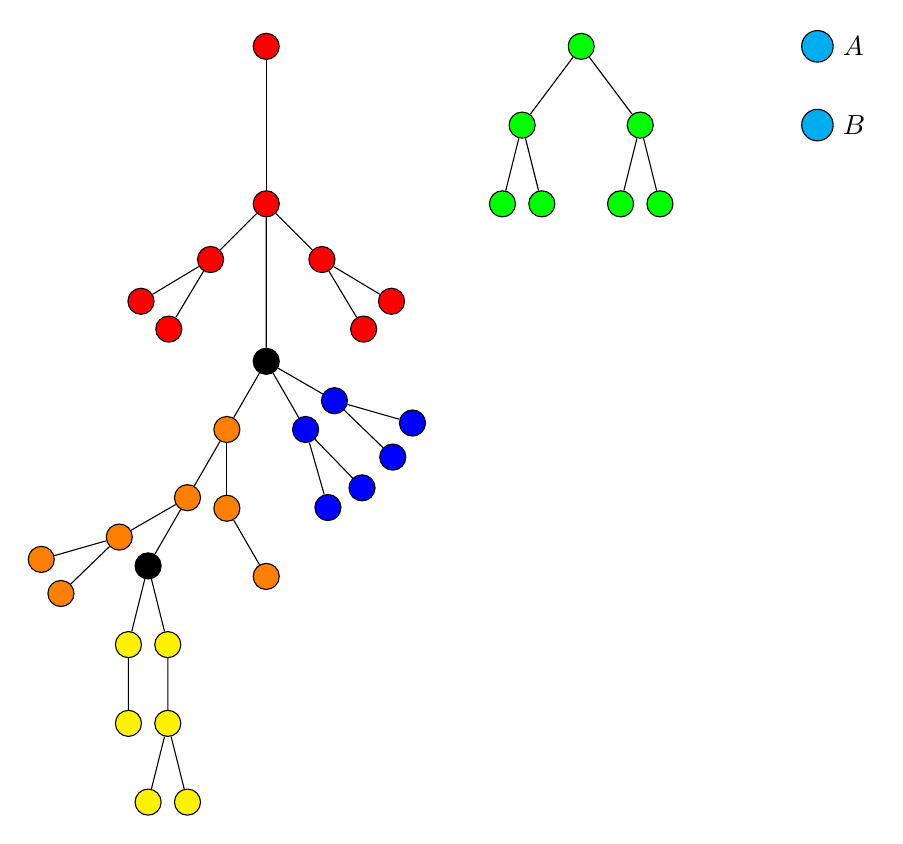
\begin{tikzpicture}
		\node[up] {}
			[level distance=20mm]
			child[grow = south] {node[up] {}
				child[grow = south west, level distance=10mm]{node[up]{}	%left up
					[sibling distance=5mm]
					child{node[up]{}}
					child{node[up]{}}
				}
				child{node[c1]{} %main up
					[sibling distance=5mm]
					child [grow = -120, level distance=10mm] {node[md]{}	%1
						child[grow = -120]{node[md]{} %2
							child[grow = -150]{node[md]{}
								child{node[md]{}}
								child{node[md]{}}
							}
							child[grow = -120]{node[c2]{} %3
								[grow = south]
								child{node[dn]{}
									child{node[dn]{}}
								}
								child{node[dn]{}
									child{node[dn]{}
										child{node[dn]{}}
										child{node[dn]{}}
									}
								}
							}
						}
						child[grow = south]{node[md]{}
							child[grow = -60]{node[md]{}}
						}
					}
					child[grow = -30, level distance=10mm]{node[ds]{}	%aux1 middle
						[sibling distance=5mm]
						child{node[ds]{}}
						child{node[ds]{}}
					}
					child [grow = -60, level distance=10mm] {node[ds]{} 	%aux2 middle
						[sibling distance=5mm]
						child{node[ds]{}}
						child{node[ds]{}}
					}
				}
				child [grow = south east, level distance=10mm] {node[up]{}	%right up
					[sibling distance=5mm]
					child{node[up]{}}
					child{node[up]{}}
				}
			}
			child[grow = east, level distance=40mm, white]{node[black, ex]{}
				[grow = south]
				[level distance=10mm]
				child[black]{node[ex]{}
					[sibling distance=5mm]
					child{node[ex]{}}
					child{node[ex]{}}
				}
				child[black] {node[ex]{}
					[sibling distance=5mm]
					child{node[ex]{}}
					child{node[ex]{}}
				}
			}
			;
			\draw [black, fill=cyan] (70mm,0) circle [radius=2mm];
			\node [right] at (72mm,0) {$A$};
			\draw [black, fill=cyan] (70mm,-10mm) circle [radius=2mm]; 
			\node [right] at (72mm,-10mm) {$B$};
	\end{tikzpicture}
\end{document}